\documentclass[aspectratio=169,11pt]{beamer}

% ---------------------------------------------------------
% APRESENTAÇÃO DO TP1 - COMPUTAÇÃO GRÁFICA / CCO
% Universidade Federal de Ouro Preto - DECOM
% Baseada em template_apresentacao_beamer.tex (professor).
%
% Compilar:  pdflatex apresentacao.tex  (duas vezes)
%
% FIGURAS: cada espaço em branco mostra o nome do arquivo esperado.
% Basta salvar o PNG com esse nome em presentation/figures/ e recompilar:
% o espaço é substituído pela imagem automaticamente.
% Tudo em VERMELHO é dado que ainda precisa ser preenchido.
% ---------------------------------------------------------

% --- PACOTES PRINCIPAIS (os do template) ---
\usepackage[utf8]{inputenc}
\usepackage[T1]{fontenc}
\IfFileExists{brazilian.ldf}{\usepackage[brazil]{babel}}{}
\usepackage{amsmath, amssymb, amsfonts}
\usepackage{booktabs}
\usepackage{tabularx}
\usepackage{graphicx}
\usepackage{xcolor}
\usepackage{hyperref}
\usepackage{listings}
\usepackage{tikz}

% --- CORES INSTITUCIONAIS / ESTILO ---
\definecolor{ufopred}{RGB}{140,29,36}
\definecolor{deepnavy}{RGB}{20,35,60}
\definecolor{lightgray}{RGB}{245,247,250}
\definecolor{darkslate}{RGB}{30,40,50}
\definecolor{softblue}{RGB}{230,238,247}

% --- TEMA BEAMER ---
\usetheme{Madrid}
\usecolortheme{default}
\setbeamertemplate{navigation symbols}{}
\setbeamercolor{structure}{fg=ufopred}
\setbeamercolor{frametitle}{fg=white,bg=ufopred}
\setbeamercolor{title}{fg=white,bg=ufopred}
\setbeamercolor{block title}{fg=white,bg=deepnavy}
\setbeamercolor{block body}{fg=black,bg=lightgray}
\setbeamercolor{alerted text}{fg=ufopred}

% --- RODAPÉ PERSONALIZADO ---
\setbeamertemplate{footline}{%
  \leavevmode%
  \hbox{%
    \begin{beamercolorbox}[wd=.72\paperwidth,ht=2.6ex,dp=1.1ex,leftskip=1.5ex]{author in head/foot}%
      \textcolor{darkslate}{\insertshorttitle}
    \end{beamercolorbox}%
    \begin{beamercolorbox}[wd=.28\paperwidth,ht=2.6ex,dp=1.1ex,rightskip=1.5ex plus1fil]{date in head/foot}%
      \hfill \textcolor{darkslate}{\insertframenumber/\inserttotalframenumber}
    \end{beamercolorbox}%
  }%
}

% --- CONFIGURAÇÃO DE CÓDIGO ---
\lstset{
  basicstyle=\ttfamily\footnotesize,
  keywordstyle=\color{ufopred}\bfseries,
  commentstyle=\color{darkslate},
  stringstyle=\color{deepnavy},
  showstringspaces=false,
  frame=single,
  rulecolor=\color{lightgray},
  breaklines=true
}

% --- COMANDOS ÚTEIS ---
\newcommand{\checkitem}{\textcolor{ufopred}{$\blacktriangleright$}}
\newcommand{\preencher}[1]{\textcolor{red}{\textbf{[#1]}}}

% Espaço de figura: {arquivo sem extensão}{rótulo}{largura (fração de \linewidth)}{altura (fração de \textheight)}
% Se figures/<arquivo>.png existir, mostra a imagem; senão, mostra o espaço em branco.
\newcommand{\figslot}[4]{%
\begin{center}
\IfFileExists{figures/#1.png}%
  {\includegraphics[width=#3\linewidth,height=#4\textheight,keepaspectratio]{figures/#1.png}}%
  {\fcolorbox{deepnavy}{lightgray}{%
    \begin{minipage}[c][#4\textheight][c]{#3\linewidth}
    \centering
    \textcolor{darkslate}{\textbf{\footnotesize #2}}\\[0.12cm]
    {\tiny\texttt{\detokenize{figures/#1.png}}}
    \end{minipage}}}%
\end{center}}

% ---------------------------------------------------------
% DADOS DA APRESENTAÇÃO
% ---------------------------------------------------------
\title[Visualização CCO - Computação Gráfica]{Visualização Geométrica, Rasterização e Recorte de Árvores Arteriais CCO}
\subtitle{BCC327 -- Computação Gráfica -- Trabalho Prático 1}
\author{João Pedro Silva Cruz \and Pedro Vítor Silva Cruz}
\institute[UFOP]{Departamento de Computação (DECOM)\\Universidade Federal de Ouro Preto (UFOP)}


% ---------------------------------------------------------
\begin{document}

\begin{frame}
  \titlepage
\end{frame}

\begin{frame}{Roteiro da Apresentação}
\tableofcontents
\end{frame}

% =========================================================
\section{Contexto e Objetivos}
% =========================================================

\begin{frame}{Contexto do Trabalho}
\begin{block}{Problema}
Uma árvore arterial CCO é só uma lista de pontos, segmentos e um raio por vaso. Como transformar esses dados em imagem? O trabalho percorre o caminho completo: do arquivo VTK até os pixels.
\end{block}

\vspace{0.25cm}

\begin{itemize}
  \item Modelos CCO fornecidos em formato \texttt{.vtk}, em 2D e em 3D.
  \item Cada vaso é um segmento, desenhado como linha ou como tubo.
  \item O atributo \texttt{raio} controla a cor e a espessura.
  \item Foco algorítmico: os algoritmos clássicos não são tratados como caixa-preta.
\end{itemize}
\end{frame}

\begin{frame}{Objetivos}
\begin{block}{Objetivo Geral}
Desenvolver uma aplicação que visualize, transforme, rasterize e recorte árvores arteriais CCO, implementando e comparando os algoritmos clássicos da disciplina.
\end{block}

\vspace{0.2cm}

\small
\begin{columns}[T]
\column{0.48\textwidth}
\begin{enumerate}
  \item Leitura, primitivas e atributos (raio $\to$ cor).
  \item Transformações, observador e projeções.
  \item Rasterização de linhas: Bresenham.
  \item Rasterização de polígonos: \emph{Scanline}.
\end{enumerate}
\column{0.48\textwidth}
\begin{enumerate}\setcounter{enumi}{4}
  \item Aliasing e antialiasing (\emph{supersampling}).
  \item Recorte de segmentos: Cohen--Sutherland, Liang--Barsky, Cyrus--Beck.
  \item Recorte de polígonos: Sutherland--Hodgman.
\end{enumerate}
\end{columns}
\end{frame}

% =========================================================
\section{Dados e Metodologia}
% =========================================================

\begin{frame}{Dados Utilizados}
\begin{columns}
\column{0.52\textwidth}
\begin{itemize}
  \item Arquivos: \texttt{dados\_modelos2D.zip} e \texttt{dados\_modelos3D.zip}.
  \item Formato: \texttt{.vtk}.
  \item Estrutura:
  \begin{itemize}
    \item pontos da geometria;
    \item células de linha (segmentos);
    \item atributo escalar \texttt{raio}.
  \end{itemize}
  \item Uma célula pode ser uma polilinha de $n$ pontos, ou seja, $n-1$ segmentos.
\end{itemize}

\column{0.44\textwidth}
\begin{block}{Modelos analisados}
\small
\begin{tabular}{lcc}
\toprule
 & \texttt{tree2D\_} & \texttt{tree3D\_}\\
 & \texttt{Nterm008} & \texttt{Nterm016}\\
\midrule
Pontos & 16 & 32\\
Segmentos & 15 & 31\\
Raio mínimo & 0,2491 & 0,2261\\
Raio máximo & 0,6668 & 0,6870\\
Dimensão & 2D & 3D\\
\bottomrule
\end{tabular}
\end{block}
\end{columns}
\end{frame}

\begin{frame}{Tecnologias Utilizadas}
\begin{itemize}
  \item Linguagem: Python 3.14.3.
  \item Janela 3D e leitura do VTK: PyVista 0.49.2 / VTK 9.7.2 (OpenGL).
  \item Matemática e algoritmos: NumPy 2.4.4 e Python puro.
  \item Figuras: Matplotlib 3.10.8. Interface: PyQt5 5.15.11 + pyvistaqt 0.13.2.
  \item Entrada: arquivos \texttt{.vtk}. Saída: visualização interativa e figuras PNG.
\end{itemize}

\vspace{0.25cm}

\begin{block}{Ambiente de execução}
\texttt{pip install -r requirements.txt} e depois \texttt{python src/main\_gui.py}. Os comandos completos estão no apêndice e no README.
\end{block}
\end{frame}

\begin{frame}{Fluxo Geral da Aplicação}
\begin{columns}[c]
\column{0.50\textwidth}
\begin{center}
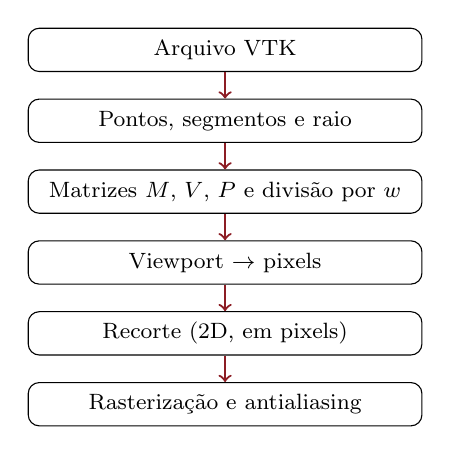
\begin{tikzpicture}[node distance=0.9cm, every node/.style={draw, rounded corners, align=center, minimum width=5.0cm, minimum height=0.55cm, font=\footnotesize}]
\node (vtk) {Arquivo VTK};
\node (mod) [below of=vtk] {Pontos, segmentos e raio};
\node (mvp) [below of=mod] {Matrizes $M$, $V$, $P$ e divisão por $w$};
\node (vp)  [below of=mvp] {Viewport $\to$ pixels};
\node (rec) [below of=vp] {Recorte (2D, em pixels)};
\node (ras) [below of=rec] {Rasterização e antialiasing};
\draw[->, thick, ufopred] (vtk) -- (mod);
\draw[->, thick, ufopred] (mod) -- (mvp);
\draw[->, thick, ufopred] (mvp) -- (vp);
\draw[->, thick, ufopred] (vp) -- (rec);
\draw[->, thick, ufopred] (rec) -- (ras);
\end{tikzpicture}
\end{center}

\column{0.46\textwidth}
\small
\begin{tabular}{@{}ll@{}}
\toprule
\textbf{Etapa} & \textbf{Arquivo}\\
\midrule
Leitura & \texttt{modelo.py}\\
$M$, $V$, $P$ & \texttt{transformacoes.py}\\
Viewport, Bresenham, & \texttt{rasterizacao.py}\\
\emph{Scanline}, SSAA & \\
Recortes & \texttt{recorte.py}\\
Figuras e demos & \texttt{didatico.py}\\
Janela 3D & \texttt{visualizador.py}\\
Interface & \texttt{main\_gui.py}\\
\bottomrule
\end{tabular}
\end{columns}
\end{frame}

\begin{frame}{O que é do grupo e o que vem de biblioteca}
\begin{columns}[T]
\column{0.49\textwidth}
\begin{block}{Implementado pelo grupo}
\small
\begin{itemize}
  \item Extração de segmentos e estatísticas.
  \item Matrizes $M$, $V$, $P$, NDC, viewport.
  \item Bresenham e DDA, \emph{framebuffer}.
  \item \emph{Scanline Fill} (ET e AET).
  \item \emph{Supersampling} e erro quadrático médio.
  \item Cohen--Sutherland, Liang--Barsky, Cyrus--Beck.
  \item Sutherland--Hodgman.
\end{itemize}
\end{block}
\column{0.49\textwidth}
\begin{block}{Com auxílio de bibliotecas}
\small
\begin{itemize}
  \item PyVista/VTK: leitura do \texttt{.vtk}, janela OpenGL, tubos, sliders, antialiasing do VTK (F2).
  \item Matplotlib: figuras e mapa de cores.
  \item PyQt5: abas, botões e console.
\end{itemize}
\vspace{0.1cm}
\footnotesize
\textcolor{ufopred}{Detalhe:} a matriz $M$ é nossa, mas é o VTK que a aplica ao desenhar; as nossas $V$ e $P$ valem na rasterização própria.
\end{block}
\end{columns}
\end{frame}

% =========================================================
\section{Implementação}
% =========================================================

\begin{frame}{Representação Geométrica e Cores}
\begin{columns}[T]
\column{0.50\textwidth}
\small
\begin{itemize}
  \item \textbf{Linhas} (espessura de tela fixa) ou \textbf{tubos} de 16 lados, com raio proporcional ao atributo.
  \item Raio por célula é interpolado para os pontos (exigência dos tubos).
  \item Rotação e escala em torno do centro do modelo.
  \item \textbf{Cor:} mapa contínuo \emph{viridis}, com $t=\frac{r-r_{\min}}{r_{\max}-r_{\min}}$.
  \item Por quê: o raio é um escalar; o \emph{viridis} é perceptualmente uniforme e legível em escala de cinza e para daltonismo.
\end{itemize}

\column{0.48\textwidth}
\figslot{vista_isometrica_persp}{Árvore 3D com tubos e cor por raio (com barra de cores)}{0.95}{0.52}
\end{columns}
\end{frame}

\begin{frame}{Transformações, Câmera e Projeções}
\small
\begin{columns}[T]
\column{0.52\textwidth}
\begin{block}{Pipeline próprio (NumPy)}
\[
\mathbf p_{\text{clip}} = P\,V\,M\,\mathbf p,\qquad
\mathbf p_{\text{NDC}}=\tfrac{(x_c,\,y_c,\,z_c)}{w_c}
\]
\[
M = T(\mathbf t)\,T(\mathbf c)\,R_zR_yR_x\,S\,T(-\mathbf c)
\]
\begin{itemize}
  \item $V$ (tipo \emph{lookAt}): mundo $\to$ câmera, que olha para $-z$.
  \item $P$: ortográfica (paralelepípedo) ou perspectiva (tronco de pirâmide, divisão por $w$).
\end{itemize}
\end{block}

\column{0.44\textwidth}
\begin{block}{O que o usuário controla}
\begin{itemize}
  \item Translação, rotação e escala (sliders).
  \item Quatro vistas: frontal, lateral, topo e isométrica.
  \item Alternância ortográfica $\leftrightarrow$ perspectiva.
  \item Impressão de $M$, $V$ e $P$ no console.
\end{itemize}
\end{block}
\footnotesize
Mundo $\neq$ câmera: mudar de vista não move o objeto, só troca a matriz $V$.
\end{columns}
\end{frame}

\begin{frame}{Módulo 3: Bresenham}
\begin{columns}[T]
\column{0.52\textwidth}
\small
\begin{itemize}
  \item Aritmética inteira, sem divisão nem ponto flutuante.
  \item $\Delta x=|x_1-x_0|$, $\Delta y=-|y_1-y_0|$, $e_0=\Delta x+\Delta y$.
  \item A cada pixel, com $e_2=2e$:
  \begin{itemize}
    \item $e_2\ge\Delta y$: $e \mathrel{+}= \Delta y$ e avança em $x$;
    \item $e_2\le\Delta x$: $e \mathrel{+}= \Delta x$ e avança em $y$.
  \end{itemize}
  \item Forma simétrica: vale nos \textbf{8 octantes}.
  \item Exemplo $(2,1)\to(13,6)$: 12 pixels $=\max(|\Delta x|,|\Delta y|)+1$.
  \item Teste: 1\,500 segmentos aleatórios (extremos, nº de pixels, conectividade, desvio $\le0{,}5$).
  \item DDA difere em 273, sempre em empates de meio pixel.
\end{itemize}

\column{0.44\textwidth}
\figslot{bresenham_exemplo}{Pixels do exemplo numérico (2,1)$\to$(13,6)}{0.95}{0.55}
\end{columns}
\end{frame}

\begin{frame}{Módulo 4: \emph{Scanline Fill}}
\begin{columns}[T]
\column{0.52\textwidth}
\small
\begin{itemize}
  \item \textbf{ET}: uma entrada por aresta não horizontal, $(y_{\min},y_{\max},x,\Delta x,\Delta y)$.
  \item \textbf{AET}: arestas que cruzam a linha atual; interseções ordenadas.
  \item Regra par-ímpar: trata polígonos côncavos.
  \item Convenções: topo exclusivo ($y_{\min}\le y<y_{\max}$) e esquerda inclusiva, para vizinhos não se sobreporem.
  \item Interseções com frações exatas.
  \item Polígono de teste côncavo: 114 pixels (área geométrica 110).
  \item Teste: 300 polígonos aleatórios iguais a um teste independente de cruzamentos.
\end{itemize}

\column{0.44\textwidth}
\figslot{scanline_exemplo}{\emph{Scanline Fill} no polígono côncavo}{0.95}{0.55}
\end{columns}
\end{frame}

\begin{frame}{Módulo 5: Aliasing e Antialiasing}
\begin{columns}[T]
\column{0.50\textwidth}
\small
\begin{itemize}
  \item Aliasing: ``escada'' de uma amostra por pixel.
  \item \textbf{Supersampling $k\times k$} (próprio): desenha em resolução $k$ vezes maior e reduz cada bloco pela média (filtro de caixa).
  \item A cor do pixel vira a fração de área coberta.
  \item Métrica: EQM contra uma referência $8\times8$.
\end{itemize}

\begin{block}{Cena de teste $64\times64$}
\small
\begin{tabular}{lcc}
\toprule
& sem AA & SSAA $4\times4$\\
\midrule
EQM & 2414,0 & 54,1\\
cores distintas & 2 & 17\\
\bottomrule
\end{tabular}
\end{block}
\footnotesize Na janela 3D, a tecla F2 liga o SSAA do VTK.

\column{0.46\textwidth}
\figslot{antialiasing_teste}{Cena de teste: sem antialiasing $\times$ SSAA $4\times4$}{0.97}{0.50}
\end{columns}
\end{frame}

\begin{frame}{Módulo 6: Recorte de Segmentos}
\begin{columns}[T]
\column{0.52\textwidth}
\small
\begin{itemize}
  \item \textbf{Cohen--Sutherland}: códigos de 4 bits; aceita ou rejeita de forma trivial; senão, recorta e repete.
  \item \textbf{Liang--Barsky}: forma paramétrica $P(u)$, com $p_ku\le q_k$ por borda; no máximo uma divisão por borda.
  \item \textbf{Cyrus--Beck}: o mesmo raciocínio com normais; serve para janela \emph{convexa} qualquer.
  \item Exemplo $(0,0)\to(12,10)$, janela $[2,10]\times[2,8]$: trecho visível $(2{,}40;\,2{,}00)\to(9{,}60;\,8{,}00)$.
  \item Cena de teste (10 segmentos): 1 aceito, 3 rejeitados, 5 recortados e 1 rejeitado só após recortar.
  \item Os três coincidem em 10 de 10; autoteste com 20\,000 casos.
\end{itemize}

\column{0.44\textwidth}
\figslot{recorte_teste}{Cena de teste: antes $\times$ depois do recorte}{0.97}{0.45}
\end{columns}
\end{frame}

\begin{frame}{Módulo 7: Recorte de Polígonos}
\begin{columns}[T]
\column{0.52\textwidth}
\small
\begin{itemize}
  \item \textbf{Sutherland--Hodgman}: uma borda da janela por vez; 4 casos por aresta (dentro--dentro, dentro--fora, fora--dentro, fora--fora).
  \item Implementado para janela convexa qualquer.
  \item Convexo: área $88\to40$.
  \item \textbf{Polígono em U} (côncavo): área $134\to32$, mas sai \emph{um} polígono com um trecho degenerado $(6,6)\!-\!(12,6)$ em vez de dois retângulos.
  \item \textbf{Weiler--Atherton}: indicado quando há côncavos, várias regiões de saída ou janelas côncavas; percorre as listas de vértices de entrada e saída. Só discutido, não implementado.
\end{itemize}

\column{0.44\textwidth}
\figslot{recorte_poligono_concavo}{Polígono em U: aresta degenerada em vermelho}{0.97}{0.45}
\end{columns}
\end{frame}

\begin{frame}{Técnicas de Computação Gráfica no TP1}
\small
\begin{tabularx}{\textwidth}{p{0.27\textwidth} X}
\toprule
\textbf{Técnica} & \textbf{Como foi utilizada no projeto}\\
\midrule
Recorte / \emph{Clipping} & Cohen--Sutherland, Liang--Barsky e Cyrus--Beck (segmentos) e Sutherland--Hodgman (polígonos), todos próprios; Weiler--Atherton apenas discutido.\\
Rasterização / Antialiasing & Bresenham (com DDA para comparação), \emph{Scanline Fill} e \emph{supersampling} próprios; SSAA do VTK na janela 3D.\\
Cor / Atributos & Mapa contínuo \emph{viridis} pelo raio; espessura pelo raio nos tubos.\\
Visibilidade, Iluminação, Ray Casting & Fora do escopo do TP1 (previstos para o TP2).\\
Transparência / Textura & Não usadas.\\
\bottomrule
\end{tabularx}
\end{frame}

% =========================================================
\section{Resultados}
% =========================================================

\begin{frame}{Observador e Projeções}
\small
\begin{columns}[T]
\column{0.24\textwidth}\figslot{vista_frontal_persp}{Frontal}{0.97}{0.22}
\column{0.24\textwidth}\figslot{vista_lateral_persp}{Lateral}{0.97}{0.22}
\column{0.24\textwidth}\figslot{vista_topo_persp}{Topo}{0.97}{0.22}
\column{0.24\textwidth}\figslot{vista_isometrica_persp}{Isométrica}{0.97}{0.22}
\end{columns}

\figslot{projecoes}{Projeção ortográfica (esq.) $\times$ perspectiva (dir.), mesma árvore e mesma vista}{0.80}{0.33}

\footnotesize Na ortográfica o tamanho não depende da distância; na perspectiva, vasos distantes encolhem (noção de profundidade, mas comprimentos distorcidos).
\end{frame}

\begin{frame}{Árvore Rasterizada, com e sem Antialiasing}
\begin{columns}[T]
\column{0.49\textwidth}
\figslot{bresenham_arvore}{Árvore rasterizada com o nosso Bresenham}{0.98}{0.50}
\column{0.49\textwidth}
\figslot{antialiasing_arvore}{Árvore sem e com SSAA $4\times4$ (com EQM)}{0.98}{0.50}
\end{columns}

\small
Modelo \texttt{tree2D\_Nterm008}. Bresenham $\times$ DDA ($600\times600$): 44 de 1\,121 pixels mudam de posição. EQM ($300\times300$) sem AA: 49,06; SSAA $4\times4$: 3,95; redução de 92\%.
\end{frame}

\begin{frame}{Recorte sobre a Árvore}
\begin{columns}[T]
\column{0.49\textwidth}
\figslot{recorte_arvore}{Recorte de segmentos: antes, depois e rasterizado}{0.98}{0.50}
\column{0.49\textwidth}
\figslot{recorte_poligono_arvore}{Estrela côncava recortada (Sutherland--Hodgman + \emph{Scanline})}{0.98}{0.50}
\end{columns}

\small
Modelo \texttt{tree2D\_Nterm008}, $300\times300$, janela $0{,}25$--$0{,}75$ da imagem. Segmentos: 7 aceitos, 3 rejeitados, 5 recortados; Cohen--Sutherland: 6 interseções; Liang--Barsky: 57 divisões; os três idênticos em 15 de 15.
\end{frame}

\begin{frame}{Validação: Autotestes}
\small
\begin{tabularx}{\textwidth}{p{0.25\textwidth} X}
\toprule
\textbf{Algoritmo} & \textbf{Teste (aleatório) e resultado}\\
\midrule
Bresenham & 1\,500 segmentos: extremos, nº de pixels, conectividade em 8 vizinhos e desvio $\le0{,}5$ pixel da reta ideal.\\
\emph{Scanline} & 300 polígonos estrelados: mesmos pixels de um teste independente de cruzamentos; vizinhos não se sobrepõem.\\
Recorte de segmentos & 20\,000 pares segmento/janela: os três algoritmos coincidem; trechos dentro da janela e sobre a reta original.\\
Sutherland--Hodgman & 600 polígonos (côncavos incluídos) $\times$ janelas aleatórias: região resultante correta; janela disjunta dá vazio.\\
\bottomrule
\end{tabularx}

\vspace{0.3cm}
Comandos: \texttt{python src/rasterizacao.py} e \texttt{python src/recorte.py}.
\end{frame}

\begin{frame}{Recurso Adicional: Interface Integrada}
\begin{columns}[T]
\column{0.46\textwidth}
\begin{block}{Recurso implementado}
\small
Interface PyQt5 que reúne todos os módulos em abas, com o 3D embutido.
\end{block}
\small
\begin{itemize}
  \item Abas: Árvore CCO, Bresenham, \emph{Scanline}, Antialiasing, Recorte e Recorte de polígonos.
  \item Bresenham interativo: clique na grade para escolher os extremos.
  \item Tabelas e estatísticas no console embutido.
  \item Exportação das 4 vistas $\times$ 2 projeções e figura ortográfica $\times$ perspectiva.
\end{itemize}

\column{0.52\textwidth}
\figslot{gui_arvore}{Captura de tela da interface (aba Árvore CCO)}{0.97}{0.58}
\end{columns}
\end{frame}

% =========================================================
\section{Discussão e Conclusão}
% =========================================================

\begin{frame}{Discussão}
\small
\begin{itemize}
  \item \textbf{Conceitos aplicados:} pipeline $M$--$V$--$P$, rasterização, antialiasing e recorte de segmentos e de polígonos.
  \item \textbf{Dificuldades:} desempate de meio pixel (Bresenham $\times$ DDA); contas exatas no \emph{Scanline}; arestas degeneradas no Sutherland--Hodgman; harmonizar a câmera do VTK com as nossas matrizes.
  \item \textbf{Biblioteca $\times$ grupo:} o VTK lê o arquivo, desenha em OpenGL, gera os tubos e monta $V$ e $P$ na janela 3D; os algoritmos pedidos são nossos.
  \item \textbf{Limitações:} sem \emph{z-buffer}; \emph{Scanline} com vértices inteiros; recorte só em 2D; Weiler--Atherton não implementado; o EQM mede a convergência para a referência $8\times8$, não o erro em relação à reta ideal.
  \item \textbf{Futuro (TP2):} visibilidade, iluminação, transparência, textura e ray casting.
\end{itemize}
\end{frame}

\begin{frame}{Conclusões}
\begin{itemize}
  \item Os sete módulos foram implementados e demonstrados sobre árvores CCO.
  \item Cada algoritmo foi conferido contra uma verificação independente, em testes aleatórios.
  \item O caso do polígono em U mostrou na prática por que o Weiler--Atherton existe.
  \item A visualização CCO é um bom exemplo de visualização científica: o atributo do vaso guia cor, espessura e recorte.
\end{itemize}

\vspace{0.25cm}

\begin{block}{Mensagem final}
Do arquivo VTK até o pixel, os algoritmos de cada passo da imagem foram implementados e testados pelo grupo; a biblioteca entra na leitura, no desenho 3D e na janela interativa.
\end{block}
\end{frame}

\begin{frame}{Referências}
\scriptsize
\begin{thebibliography}{99}
\bibitem{foley} FOLEY, J. D. et al. \textit{Computer Graphics: Principles and Practice}. 2. ed. Addison-Wesley, 1990.
\bibitem{schreiner1993} SCHREINER, W.; BUXBAUM, P. Computer-optimization of vascular trees. \textit{IEEE Transactions on Biomedical Engineering}, v. 40, n. 5, 1993.
\bibitem{karch} KARCH, R. et al. A three-dimensional model for arterial tree representation, generated by constrained constructive optimization. \textit{Computers in Biology and Medicine}, v. 29, n. 1, 1999.
\bibitem{bres} BRESENHAM, J. E. Algorithm for computer control of a digital plotter. \textit{IBM Systems Journal}, v. 4, n. 1, 1965.
\bibitem{lb} LIANG, Y.-D.; BARSKY, B. A. A new concept and method for line clipping. \textit{ACM Transactions on Graphics}, v. 3, n. 1, 1984.
\bibitem{cb} CYRUS, M.; BECK, J. Generalized two- and three-dimensional clipping. \textit{Computers \& Graphics}, v. 3, n. 1, 1978.
\bibitem{sh} SUTHERLAND, I. E.; HODGMAN, G. W. Reentrant polygon clipping. \textit{Communications of the ACM}, v. 17, n. 1, 1974.
\bibitem{wa} WEILER, K.; ATHERTON, P. Hidden surface removal using polygon area sorting. \textit{ACM SIGGRAPH Computer Graphics}, v. 11, n. 2, 1977.
\bibitem{vtk} VTK Documentation. \url{https://vtk.org/}. PyVista: \url{https://pyvista.org/}.
\end{thebibliography}
\end{frame}

% ---------------------------------------------------------
\appendix
\section{Apêndice}

\begin{frame}{Bresenham nos 8 octantes}
\figslot{bresenham_octantes}{Segmentos nos oito octantes (linha preta: reta ideal)}{0.55}{0.62}
\end{frame}

\begin{frame}{Scanline e Sutherland--Hodgman: detalhes}
\begin{columns}[T]
\column{0.49\textwidth}
\figslot{scanline_roi}{Região de interesse preenchida sobre a árvore}{0.98}{0.50}
\column{0.49\textwidth}
\figslot{recorte_poligono_passos}{Sutherland--Hodgman passo a passo, uma borda por vez}{0.98}{0.50}
\end{columns}
\end{frame}

\begin{frame}[fragile]{Comandos de Execução}
\begin{lstlisting}[language=bash]
pip install -r requirements.txt
python src/main_gui.py                      # interface integrada
python src/visualizador.py ARQUIVO.vtk --info
python src/didatico.py bresenham --arvore ARQUIVO.vtk
python src/didatico.py antialiasing --arvore ARQUIVO.vtk --k 4 --ref 8
python src/didatico.py recorte --arvore ARQUIVO.vtk --janela 0.25 0.25 0.75 0.75
python src/didatico.py recorte-poligonos --arvore ARQUIVO.vtk
python src/rasterizacao.py && python src/recorte.py   # autotestes
\end{lstlisting}

\begin{block}{Observação}
\small
Modelos esperados em \texttt{data/dados\_modelos2D/} e \texttt{data/dados\_modelos3D/}. O README traz o roteiro completo de teste.
\end{block}
\end{frame}

\begin{frame}{Obrigado!}
\begin{center}
{\Huge Obrigado!}
\end{center}
\end{frame}

\end{document}